\documentclass[tikz,border=6pt]{standalone}
\usetikzlibrary{decorations.pathmorphing,intersections,spath3}
\begin{document}
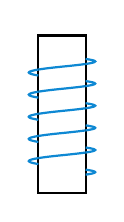
\begin{tikzpicture}[thick]
  \def\pgfintersectiontolerance{0.01pt}
  \path[
    decorate,
    decoration={coil,amplitude=12pt,segment length=8pt,aspect=.01},
    spath/save=spring
  ] (0,-.95) -- (0,1.1);
  \path[spath/save=rod] (-.3,-1) rectangle (.3,1);
  \draw[black,spath/use=rod];
  \tikzset{
    spath/replace lines=rod,
    spath/split at intersections with={spring}{rod},
    spath/get components of={spring}\parts
  }
  \foreach \k in {4,6,7,8,10,11,12,14,15,16,18,19,20,22,23,24} {
    \edef\p{\getComponentOf\parts{\k}}
    \draw[cyan!70!blue,spath/use=\p];
  }
\end{tikzpicture}
\end{document}
